\graphicspath{{content/chapters/4_results/figures/}}

\chapter{Results and Discussion}%
\label{chp:results}

In this chapter, we will present the results of all our replications and
experiments. The chapter is structured as follows:
Section~\ref{sec:replication} presents the results of our replicated models
when evaluated on a dataset used by the original authors. These results are
presented beside the results of the original work to illustrate the
similarities in the figures, confirming successful replication. The remainder
of the sections in the chapter present the results of the experiments carried
out as part of the methodology proposed in the previous chapter.
Section~\ref{sec:agg_res_cat} presents the metrics discussed in
Section~\ref{sec:metrics} aggregated over all the variants and classes in the
first and second phases specified in Section~\ref{sec:variants}, which take
attack categories as the target label. Section~\ref{sec:agg_res_att} presents
the same information, considering instead the third and fourth phases defined
in Section~\ref{sec:variants}, which take the individual attack name as the
target label. More information about the methods of aggregation applied is
specified in these sections. Section~\ref{sec:res_var_cat} presents heatmaps
that indicate the recall values of each variant in the discussed in
Section~\ref{sec:variants} on each label class. The predictions of each
combination of model and variant are available in pickle format in the
`results' folder on this project's GitHub repository~\cite{repo}.

\section{Replication}%
\label{sec:replication}

As discussed in the previous chapter, each model considered is evaluated on a
dataset used by the original authors to verify it was replicated correctly.
More specifically, the supervised models are evaluated on the CSE-CIC-IDS2018
dataset whilst the unsupervised models are evaluated on the NSL-KDD dataset.
The evaluation methodology is also applied to two of the models and the dataset
originally used by Kus et al.~\cite{Kus}, to verify its correct replication.
All the models we set out to replicate were successfully replicated with the
exception of the AdaBoost model. Our attempts to replicate this model yielded
poor results that did not compare to those of Karatas et al.~\cite{Karatas}.

Tables~\ref{tab:karatas_rep_agg} and~\ref{tab:karatas_rep_acc} display the
results of the replication of the work of Karatas et al.~\cite{Karatas}. These
are the metrics used by the original authors calculated from the predictions of
the models trained on the CSE-CIC-IDS2018 dataset. A stratified sample of the
dataset with no omitted attacks was employed during training and testing to
match the original work as closely as possible. In the same tables are the
results presented in the original work. Analysing these results, we can
conclude that the differences are negligible and can be amounted to the
stochasticity of the training and testing process. Therefore, we conclude that
the five supervised models presented were replicated successfully.
%
\begin{table}
    \caption{Karatas et al.~\cite{Karatas} replication aggregate results\label{tab:karatas_rep_agg}}
    \centering
    \begin{tblr}{|c|c|c|c|c|c|c|}
        \hline
        \SetCell[c=5]{m} \textbf{Our Results}                         \\
        \hline
        \textbf{Algorithm} & \textbf{Accuracy}  & \textbf{Recall}
                           & \textbf{Precision} & \textbf{F1-Measure} \\
        \hline
        \gls{dt}           & 0.99               & 0.97
                           & 0.94               & 0.95                \\
        \gls{rf}           & 0.99               & 0.94
                           & 0.95               & 0.95                \\
        \gls{gb}           & 0.99               & 1.00
                           & 0.96               & 0.98                \\
        \gls{knn}          & 0.97               & 0.91
                           & 0.71               & 0.76                \\
        \gls{lda}          & 0.88               & 0.89
                           & 0.52               & 0.57                \\
        \hline
        \SetCell[c=5]{m} \textbf{Original Authors' Results}           \\
        \hline
        \textbf{Algorithm} & \textbf{Accuracy}  & \textbf{Recall}
                           & \textbf{Precision} & \textbf{F1-Measure} \\
        \hline
        \gls{dt}           & 0.996              & 0.996
                           & 0.996              & 0.996               \\
        \gls{rf}           & 0.994              & 0.993
                           & 0.994              & 0.996               \\
        \gls{gb}           & 0.993              & 0.993
                           & 0.993              & 0.993               \\
        \gls{knn}          & 0.981              & 0.981
                           & 0.979              & 0.980               \\
        \gls{lda}          & 0.912              & 0.912
                           & 0.920              & 0.916               \\
        \hline
    \end{tblr}
\end{table}

%
\begin{table}
    \caption{Karatas et al.~\cite{Karatas} replication accuracy per class\label{tab:karatas_rep_acc}}
    \centering
    \begin{tblr}{|c|c|c|c|c|c|c|}
        \hline
        \SetCell[c=7]{m} \textbf{Our Results}                                  \\
        \hline
        \textbf{Algorithm} & \textbf{Benign}      & \textbf{Bot}       &
        \textbf{\gls{dos}} & \textbf{Brute Force} & \textbf{Injection} &
        \textbf{Infiltration}                                                  \\
        \hline
        \gls{dt}           & 0.993                & 1.000              & 1.000
                           & 1.000                & 0.805              & 1.000 \\
        \gls{rf}           & 0.991                & 1.000              & 1.000
                           & 1.000                & 0.747              & 0.917 \\
        \gls{gb}           & 0.991                & 1.000              & 1.000
                           & 1.000                & 0.987              & 1.000 \\
        \gls{knn}          & 0.970                & 1.000              & 1.000
                           & 1.000                & 0.490              & 1.000 \\
        \gls{lda}          & 0.840                & 1.000              & 1.000
                           & 0.961                & 0.626              & 0.917 \\
        \hline
        \SetCell[c=7]{m} \textbf{Original Authors' Results}                    \\
        \hline
        \textbf{Algorithm} & \textbf{Benign}      & \textbf{Bot}       &
        \textbf{\gls{dos}} & \textbf{Brute Force} & \textbf{Injection} &
        \textbf{Infiltration}                                                  \\
        \hline
        \gls{dt}           & 0.996                & 1.000              & 1.000
                           & 1.000                & 0.962              & 0.856 \\
        \gls{rf}           & 0.995                & 1.000              & 1.000
                           & 1.000                & 1.000              & 0.927 \\
        \gls{gb}           & 0.989                & 1.000              & 1.000
                           & 0.996                & 1.000              & 0.978 \\
        \gls{knn}          & 0.981                & 1.000              & 1.000
                           & 0.999                & 1.000              & 0.739 \\  % TODO: there is a risk infiltration and injection had their encodings switched
        \gls{lda}          & 0.863                & 0.984              & 0.999
                           & 0.518                & 0.674              & 0.978 \\
        \hline
    \end{tblr}
\end{table}

Figure~\ref{fig:pu_rep} shows the results of the replication of the work of Pu
et al.~\cite{Pu} in the form of the \gls{roc} curve of the replicated model.
This model was trained and tested on the complete NSL-KDD dataset preprocessed
according to the methodology of the original authors. This curve can be
compared to the curve presented by the original authors to verify the
replication of the model. The right image in the figure is the image presented
by the original authors, with the red line representing the proposed model,
\gls{ssc}-\gls{ocsvm}. Comparing the two curves, the performance of our
replicated model is similar to that of the original authors, and hence we
conclude the model was successfully replicated.

\begin{figure}[htbp]
    \centering
    \begin{minipage}[h]{0.5\textwidth}
        \centering
        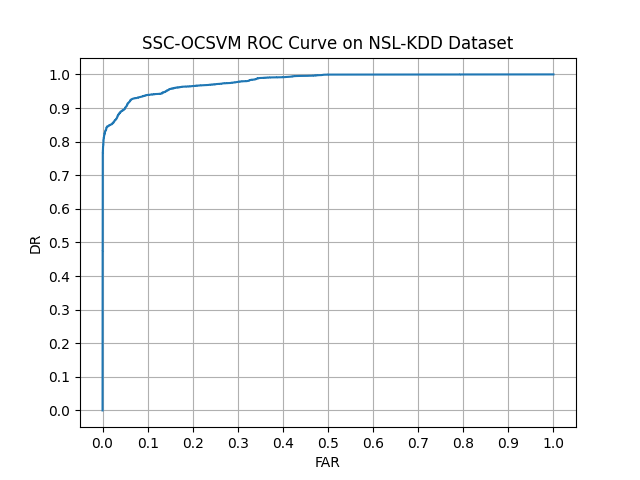
\includegraphics[width=\textwidth,keepaspectratio]{mixed_roc}
    \end{minipage}\hfill
    \begin{minipage}[h]{0.5\textwidth}
        \centering
        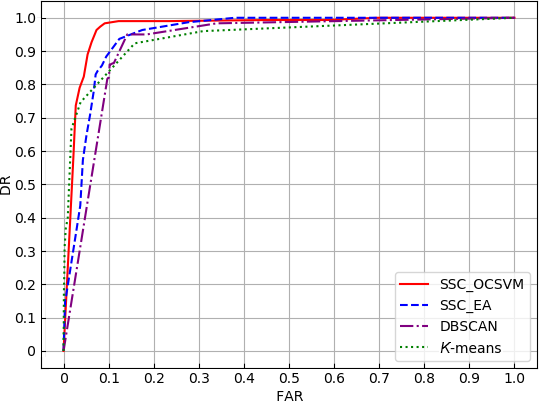
\includegraphics[width=\textwidth,keepaspectratio]{mixed_roc_original}
    \end{minipage}
    \caption[Pu et al.\ replication ROC curve]{The ROC curve of our replicated \gls{ssc}-\gls{ocsvm} model (left) compared to that of the original author (right).\label{fig:pu_rep}}
\end{figure}

Table~\ref{tab:cao_rep} shows the results of the replication of the work of Cao
et al.~\cite{Cao}. These figures represent the \gls{auc-roc} per class
calculated from the predictions of the model when trained on the complete
NSL-KDD dataset. The preprocessing pipeline applied consists of the same steps
proposed by Cao et al.~\cite{Cao}. Comparing the \gls{auc-roc} scores of our
replicated model with the original work, we observe negligible differences
which can be attributed to the stochasticity of the training and testing
process. Hence, we conclude the model was successfully replicated.
%m
\begin{table}
    \caption{Cao et al.~\cite{Cao} replication \gls{auc-roc} per class\label{tab:cao_rep}}
    \centering
    \begin{tblr}{|c|c|c|c|c|}
        \hline
        \SetCell[c=5]{m} \textbf{Our Results}                 \\
        \hline
        \textbf{Algorithm}    & \textbf{Probe} &
        \textbf{\gls{dos}}    & \textbf{R2L}   & \textbf{U2R}
        \\
        \hline
        \gls{sae}-\gls{ocsvm} & 0.975          & 0.972
                              & 0.926          & 0.959
        \\
        \hline
        \SetCell[c=5]{m} \textbf{Original Authors' Results}   \\
        \hline
        \gls{sae}-\gls{ocsvm} & 0.987          & 0.972
                              & 0.923          & 0.948
        \\
        \hline
    \end{tblr}
\end{table}

Figures~\ref{fig:kus_rep_cat} and~\ref{fig:kus_rep_att} show the results of the
replication of the work of Kus et al.~\cite{Kus}. Note, only the \gls{rf} model
results are presented. The \gls{svm} and \gls{bilstm} models were also
replicated, however these results are not presented due to space constraints.
The methodology of Kus et al.~\cite{Kus} is consistent across all models and
hence, these results are sufficient to confirm the validity of the replication.
These figures represent heatmaps indicating the per class recall values of each training
variant. Each row represents the per class recall values of a particular
variant whereas each column represents the recall values of each variant on the
instances of a particular class. The heatmaps presented are those of our
replication. Unlike the previous replications, we cannot present the results of
Kus et al.~\cite{Kus} here due to space limitations, however these can be found
in the original paper. 

Note, the label encodings used by our replication is
different to that of the original authors, hence, the columns of the heatmaps
appear to be shuffled. The encoding zero represents the benign class in both
our replication and the original work. Analysing the heatmaps, we observe near
identical patterns in our replication when compared to the original results.
Hence, we can conclude our implementation accurately replicates the methodology
proposed by Kus et al.~\cite{Kus}.
%
\begin{figure}[htbp]
    \centering
    \begin{minipage}[h]{0.5\textwidth}
        \centering
        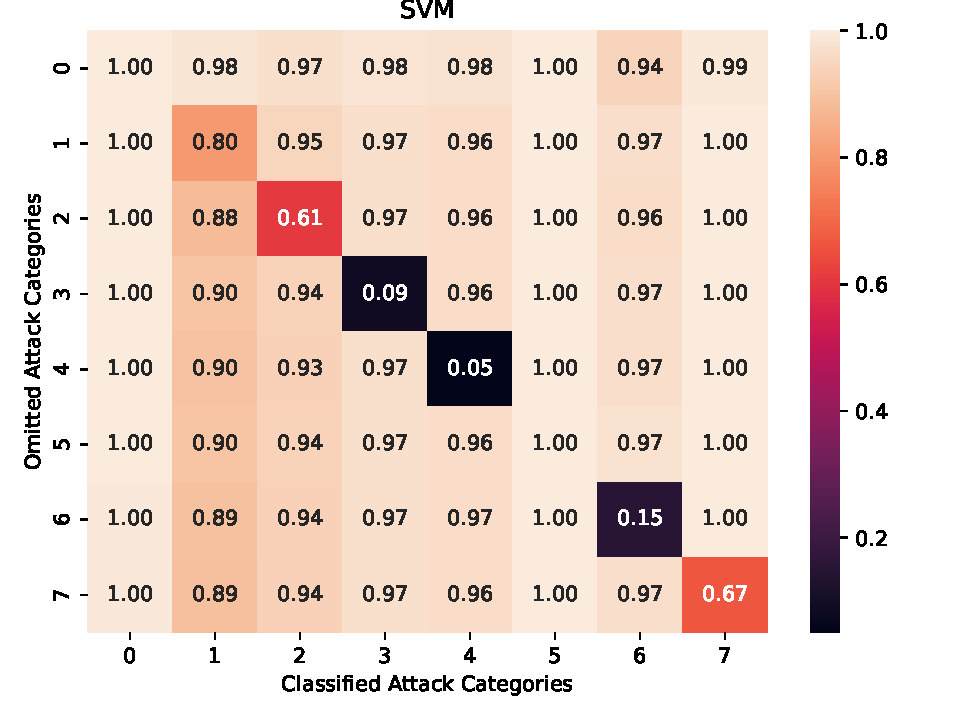
\includegraphics[width=\textwidth,keepaspectratio]{kus_rf_exc_category}
    \end{minipage}\hfill
    \begin{minipage}[h]{0.5\textwidth}
        \centering
        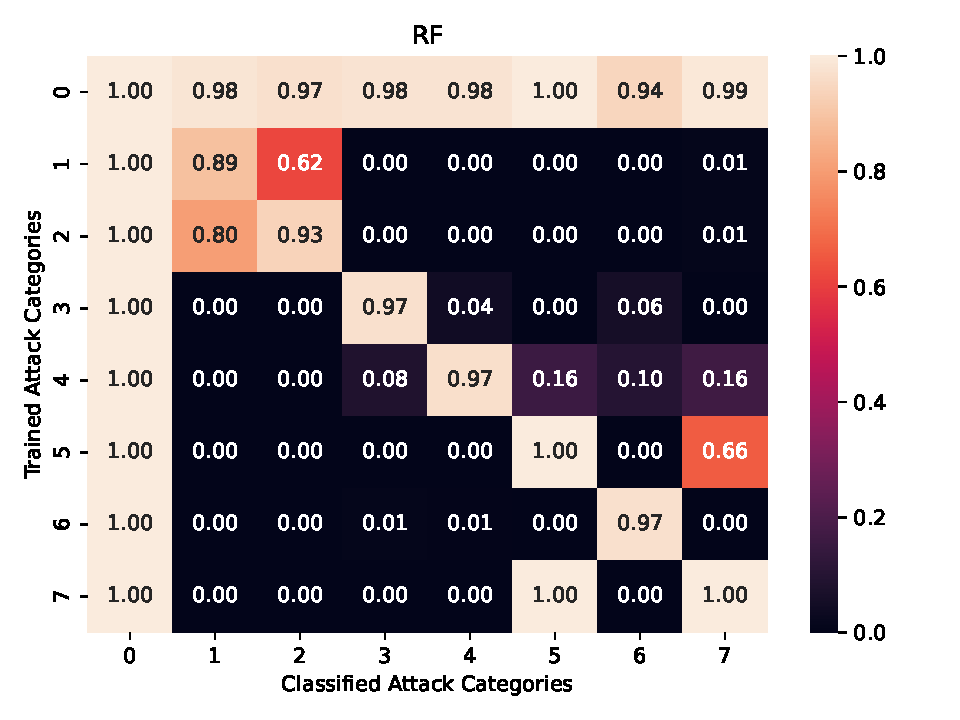
\includegraphics[width=\textwidth,keepaspectratio]{kus_rf_inc_category}
    \end{minipage}
    \caption[Kus et al.~\cite{Kus} Replication Category Heatmaps]{Kus et al.~\cite{Kus} replication heatmaps illustrating recall per category on each training variant\label{fig:kus_rep_cat}}
\end{figure}

\begin{figure}[htbp]
    \centering
    \begin{minipage}[h]{0.5\textwidth}
        \centering
        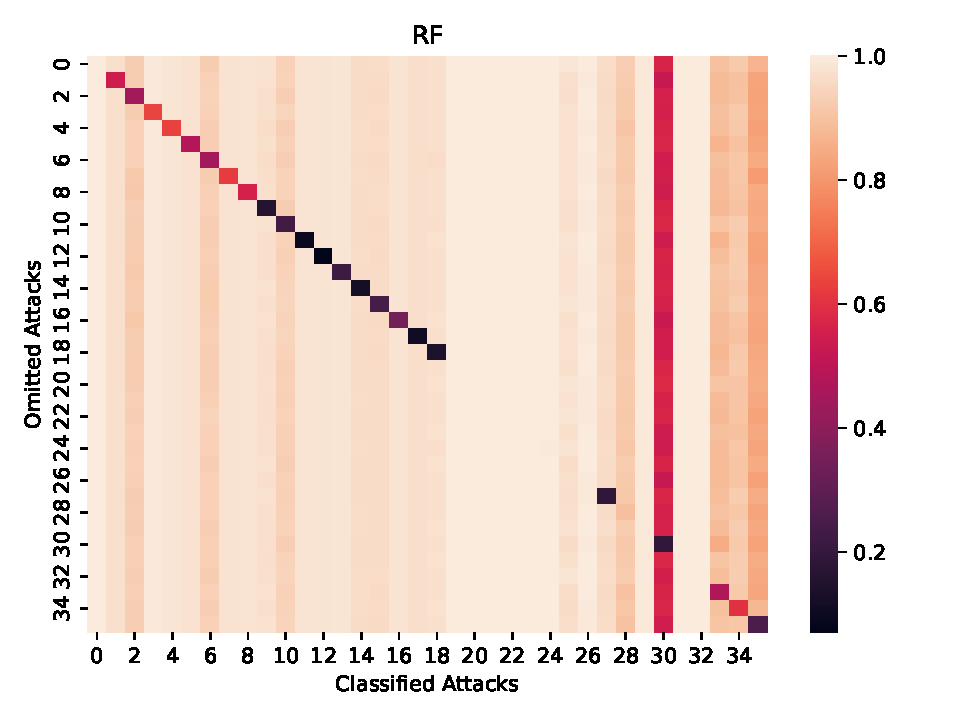
\includegraphics[width=\textwidth,keepaspectratio]{kus_rf_exc_attack}
    \end{minipage}\hfill
    \begin{minipage}[h]{0.5\textwidth}
        \centering
        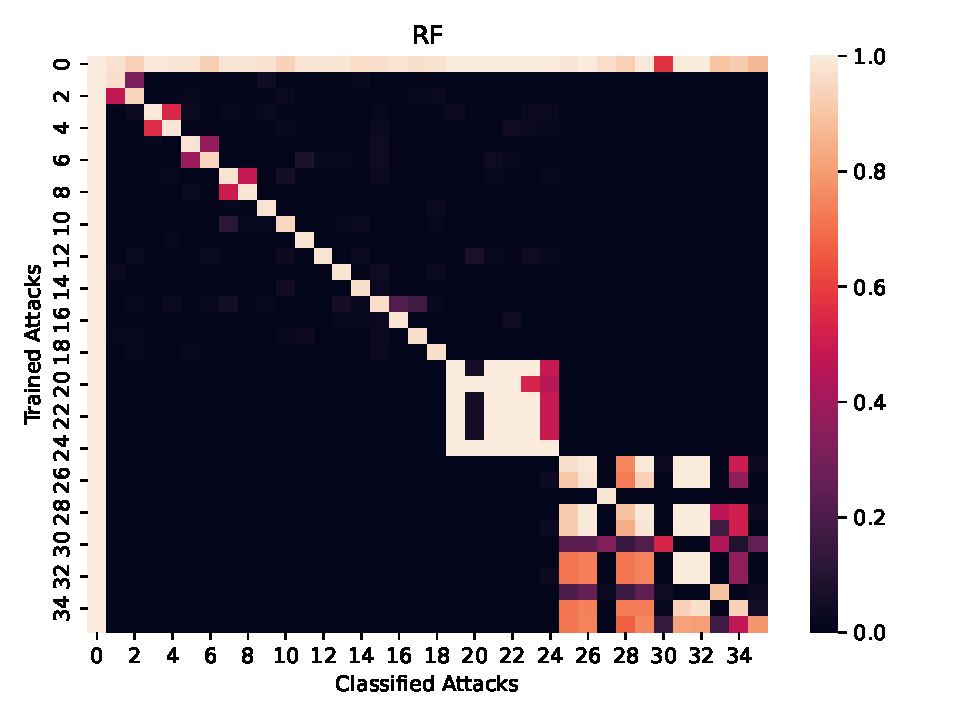
\includegraphics[width=\textwidth,keepaspectratio]{kus_rf_inc_attack}
    \end{minipage}
    \caption[Kus et al.~\cite{Kus} Replication Individual Attack Heatmaps]{Kus et al.~\cite{Kus} replication heatmaps illustrating recall for each individual attack on each training variant\label{fig:kus_rep_att}}
\end{figure}

% \begin{figure}[htbp]
%     \centering
%     \begin{minipage}[h]{0.5\textwidth}
%         \centering
%         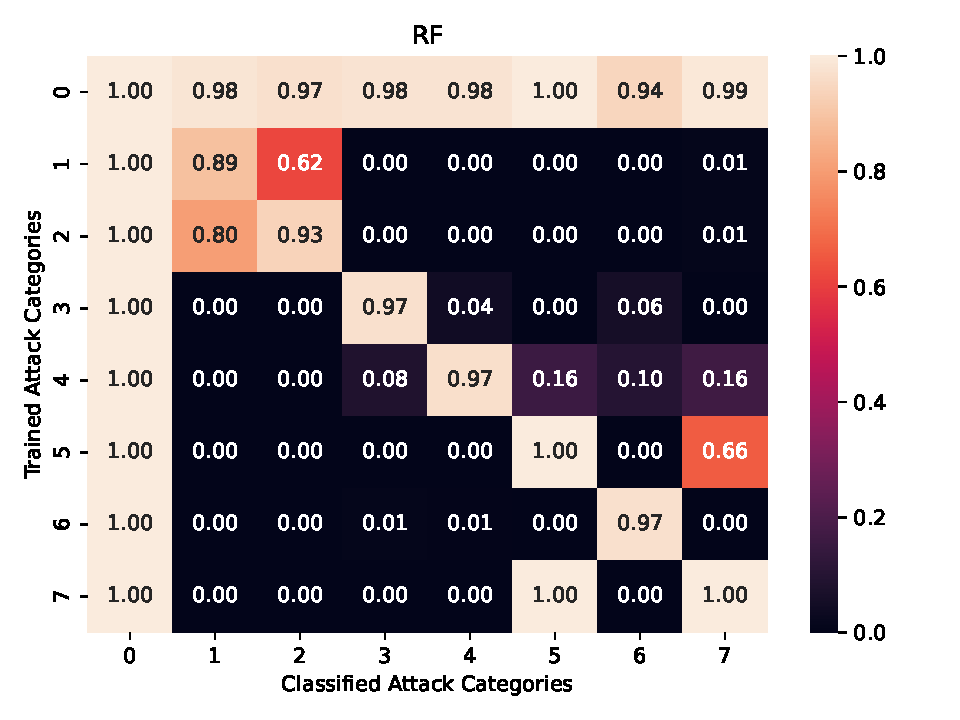
\includegraphics[width=\textwidth,keepaspectratio]{kus_rf_inc_category}
%     \end{minipage}\hfill
%     \begin{minipage}[h]{0.5\textwidth}
%         \centering
%         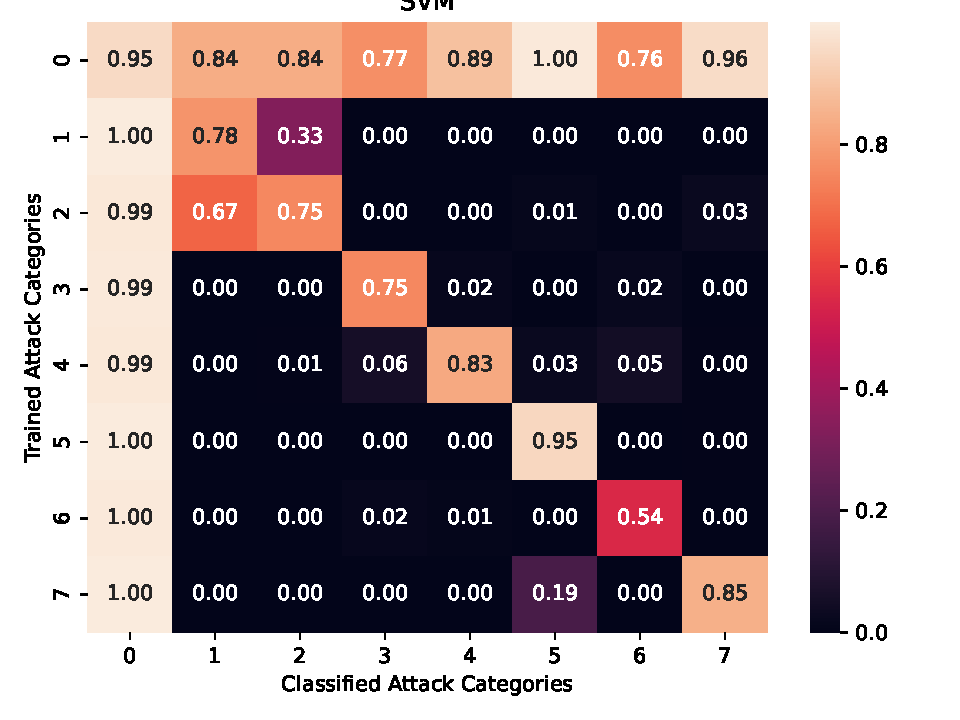
\includegraphics[width=\textwidth,keepaspectratio]{kus_svm_inc_category}
%     \end{minipage}
% \begin{minipage}[h]{0.3\textwidth}
%     \centering
%     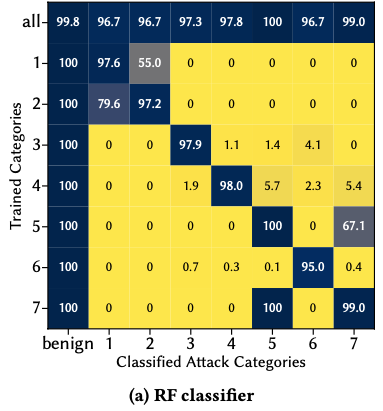
\includegraphics[width=\textwidth,keepaspectratio]{kus_rf_inc_category_original}
% \end{minipage}\hfill
% \begin{minipage}[h]{0.3\textwidth}
%     \centering
%     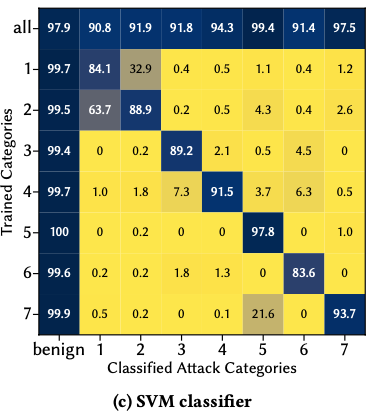
\includegraphics[width=\textwidth,keepaspectratio]{kus_svm_inc_category_original}
% \end{minipage}
%     \caption[Kus et al.~\cite{Kus} Replication Single Category Heatmaps]{Kus et al.~\cite{Kus} replication heatmaps illustrating recall per category against trained category\label{fig:kus_rep_inc_cat}}
% \end{figure}

% \begin{figure}[htbp]
%     \centering
%     \begin{minipage}[h]{0.5\textwidth}
%         \centering
%         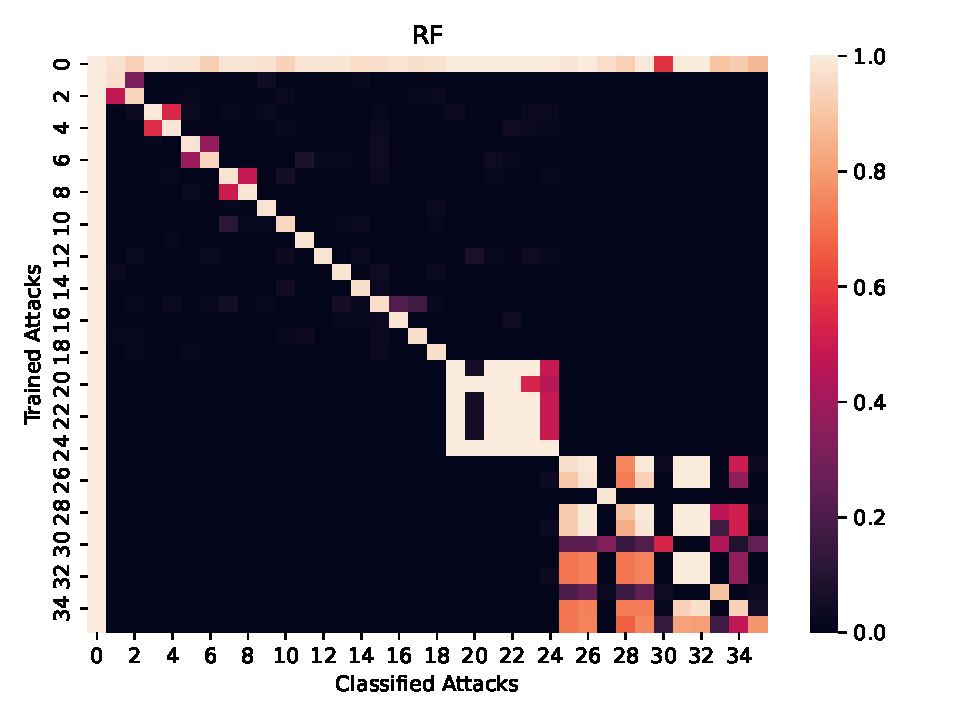
\includegraphics[width=\textwidth,keepaspectratio]{kus_rf_inc_attack}
%     \end{minipage}\hfill
%     \begin{minipage}[h]{0.5\textwidth}
%         \centering
%         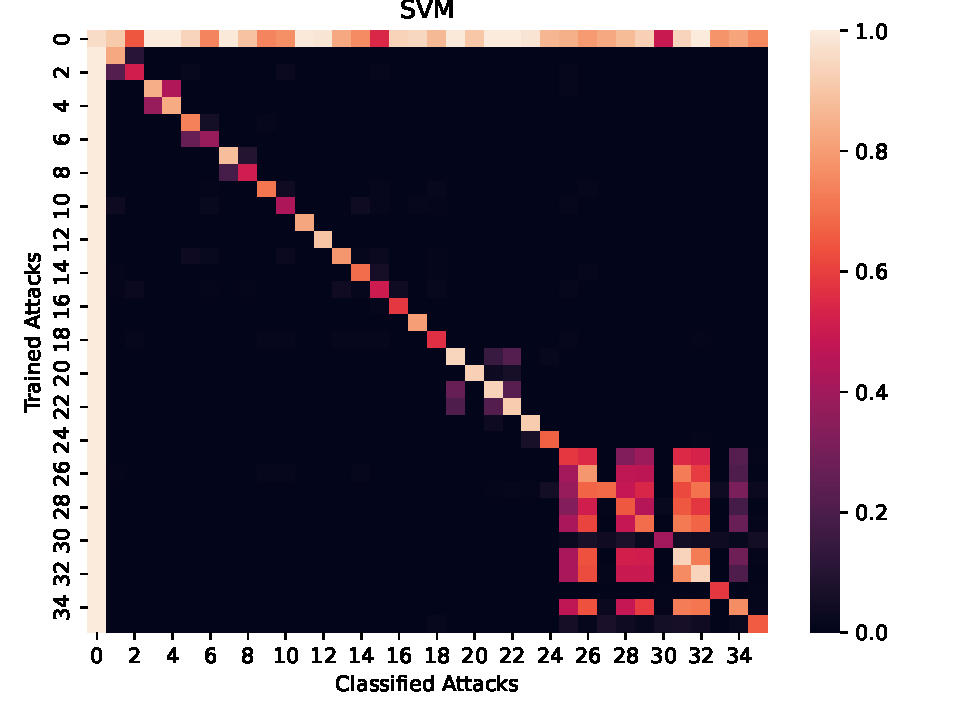
\includegraphics[width=\textwidth,keepaspectratio]{kus_svm_inc_attack}
%     \end{minipage}
% \begin{minipage}[h]{0.3\textwidth}
%     \centering
%     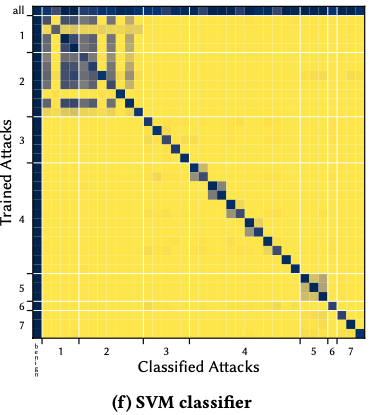
\includegraphics[width=\textwidth,keepaspectratio]{kus_rf_inc_attack_original}
% \end{minipage}\hfill
% \begin{minipage}[h]{0.3\textwidth}
%     \centering
%     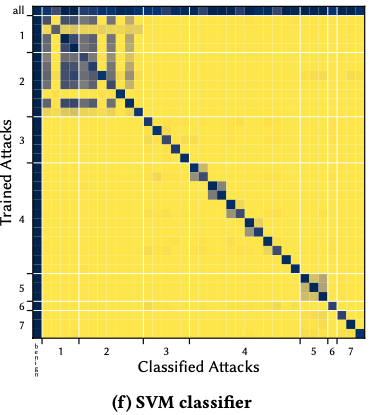
\includegraphics[width=\textwidth,keepaspectratio]{kus_svm_inc_attack_original}
% \end{minipage}
%     \caption[Kus et al.~\cite{Kus} Replication Single Attack Heatmaps]{Kus et al.~\cite{Kus} replication heatmaps illustrating recall per attack against trained attack\label{fig:kus_rep_inc_att}}
% \end{figure}
% 

\section{Aggregate Results Omitting Categories}%
\label{sec:agg_res_cat}

The aggregate results of all the experiments are shown in
Table~\ref{tab:results_cat_agg}.

The methodology described in the previous chapter yields these metrics for each
variant and class. To better interpret the overall performance of each model
and address \hyperlink{obj}{Objective 1} we present the average of all these
metrics, considering only variants of Phase 1 discussed in
Section~\ref{sec:variants}, which exclude attack categories. These variants
were selected to generate the aggregate results as they offer the most
realistic simulation of a practical scenario whereby an unknown attack is
deployed on a model trained on several categories of known attacks.

The unsupervised models were trained on only one variant as all variants are
rendered identical following their preprocessing pipelines, which involve
removing all malicious samples. Hence, the above discussed averaging does not
apply to these models. Both supervised and unsupervised models, however,
generate metrics per label class. The macro-average, which is a non-weighted
average, is presented when aggregating across classes to reduce the impact of
class imbalance.

% category
\begin{table}
    \caption{Aggregate results when excluding
        categories\label{tab:results_cat_agg}}
    \centering
    \begin{tblr}{|c|c|c|c|c|c|c|}
        \hline
        \textbf{Algorithm}    & \textbf{Accuracy}  & \textbf{Recall}     &
        \textbf{Recall-Unk}   & \textbf{Precision} & \textbf{F1-Measure}         \\
        \hline
        \gls{dt}              & 0.962              & 0.828               & 0.134
                              & 0.942              & 0.832                       \\
        \gls{rf}              & 0.964              & 0.830               & 0.228
                              & 0.910              & 0.848                       \\
        \gls{gb}              & 0.948              & 0.804               & 0.118
                              & 0.872              & 0.800                       \\
        \gls{knn}             & 0.958              & 0.800               & 0.248
                              & 0.900              & 0.796                       \\
        \gls{lda}             & 0.914              & 0.766               & 0.564
                              & 0.850              & 0.718                       \\
        \gls{ssc}-\gls{ocsvm} & 0.760              & 0.590               & 0.554
                              & 0.820              & 0.670                       \\
        \gls{sae}-\gls{ocsvm} & 0.800              & 0.640               & 0.600
                              & 0.830              & 0.650                       \\ % & 0.825 (AUC)
        \hline
    \end{tblr}
\end{table}

The results of the supervised models are generally high indicating a good
ability to detect known attacks from network data, with the \gls{dt} and
\gls{rf} models performing slightly better than the other models. However, this
degrades significantly in the face of unknown attacks. This is indicated by the
low values in the Recall-Unk column for all models except for \gls{lda}. This
indicates a very low ability to generalise to unknown attack categories in
these models. The \gls{lda} model stands out from the other supervised models,
exhibiting a significantly higher Recall-Unk value, comparable to those of the
unsupervised models. The value is still significantly lower than those of known
attacks, however is an impressive value nonetheless due to the inherent
difficulty in detecting unknown attacks.

The unsupervised models on the other hand exhibit a less significant difference
between their recall and Recall-Unk values, however have a lower recall value
than the supervised models. The accuracies and F1-scores of the models are also
lower indicating worse overall performance when compared to the supervised
models. The accuracies stand at 76\% and 80\% which are notable figures,
however, as previously discussed, accuracy may be skewed by a large number of
correct benign predictions. Hence, the recalls and F1-scores may be more
significant given the class imbalance present in the dataset. Considering the
recalls and F1-scores in Table~\ref{tab:results_cat_agg}, the unsupervised
models could certainly provide valuable information, however may miss a
significant number of attacks.

Comparing the \gls{ssc}-\gls{ocsvm} model to the \gls{sae}-\gls{ocsvm} model,
the performance figures are quite similar, indicating \gls{dl} may not suffer
the same inefficacy discovered by Zoppi et al.~\cite{Zoppi} when considering
unsupervised models.

\begin{table}
    \caption{Accuracy per class when excluding
        categories\label{tab:results_cat_acc}}
    \centering
    \begin{tblr}{|c|c|c|c|c|c|c|}
        \hline
        \textbf{Algorithm}    & \textbf{Benign}      & \textbf{Bot}       &
        \textbf{\gls{dos}}    & \textbf{Brute Force} & \textbf{Injection} &
        \textbf{Infiltration}                                                     \\
        \hline
        \gls{dt}              & 0.990                & 0.971              & 0.849
                              & 0.902                & 0.938              & 0.440 \\
        \gls{rf}              & 0.994                & 0.802              & 0.815
                              & 0.902                & 0.862              & 0.448 \\
        \gls{gb}              & 0.989                & 0.741              & 0.622
                              & 0.751                & 0.754              & 0.240 \\
        \gls{knn}             & 0.985                & 0.801              & 0.831
                              & 0.920                & 0.892              & 0.388 \\
        \gls{lda}             & 0.940                & 0.773              & 0.805
                              & 0.951                & 0.954              & 0.162 \\
        \gls{ssc}-\gls{ocsvm} & 0.772                & 0.006              & 0.778
                              & 0.999                & 0.667              & 0.313 \\
        \gls{sae}-\gls{ocsvm} & 0.818                & 0.496              & 0.734
                              & 0.999                & 0.384              & 0.391 \\
        \hline
    \end{tblr}
\end{table}

\begin{table}
    \caption{F1-Measure per class when excluding
        categories\label{tab:results_cat_f1}}
    \centering
    \begin{tblr}{|c|c|c|c|c|c|c|}
        \hline
        \textbf{Algorithm}    & \textbf{Benign}      & \textbf{Bot}       &
        \textbf{\gls{dos}}    & \textbf{Brute Force} & \textbf{Injection} &
        \textbf{Infiltration}                                                     \\
        \hline
        \gls{dt}              & 0.978                & 0.734              & 0.878
                              & 0.936                & 0.964              & 0.568
        \\
        \gls{rf}              & 0.978                & 0.670              & 0.828
                              & 0.936                & 0.894              & 0.576
        \\
        \gls{gb}              & 0.962                & 0.508              & 0.644
                              & 0.772                & 0.774              & 0.368
        \\
        \gls{knn}             & 0.974                & 0.554              & 0.856
                              & 0.950                & 0.926              & 0.522
        \\
        \gls{lda}             & 0.948                & 0.252              & 0.892
                              & 0.972                & 0.974              & 0.276
        \\
        \gls{ssc}-\gls{ocsvm} & 0.850                & 0.000              & 0.880
                              & 1.000                & 0.800              & 0.480
        \\
        \gls{sae}-\gls{ocsvm} & 0.870                & 0.070              & 0.850
                              & 1.000                & 0.560              & 0.560
        \\
        \hline
    \end{tblr}
\end{table}

Table~\ref{tab:results_cat_acc} presents the aggregate per class accuracy
calculated by averaging the per class accuracies of each variant where an
attack category is omitted. Table~\ref{tab:results_cat_f1} contains the per
class F1-scores averaged across the same variants.

Analysing the results of these tables, we can further investigate the behaviour
of the models. Firstly, we note that some attack categories appear to be more
difficult to predict than others. For instance, the `Infiltration' category
exhibits lower accuracy across all models. A potential explanation for this is
that `Infiltration' is a broad category involving the exploitation of software
that can take a wide variety of forms. Hence, `Infiltration' attacks may differ
significantly among themselves making it more difficult for the model to learn
common patterns. Additionally, the dataset only contains five attacks under
this category, with a relatively small number of instances compared to most
other categories, potentially aggravating the issue. Another potential
explanation may be that `Infiltration' attacks resemble benign traffic more
closely than other categories, rendering themselves difficult to distinguish
from normal traffic.

The comparison of the unsupervised model with the supervised models in
Table~\ref{tab:results_cat_acc} and Table~\ref{tab:results_cat_f1} reveals an
interesting phenomenon. Whilst the unsupervised models perform far worse
overall, they seem to perform very similarly to the supervised models on
certain categories. The models exhibit low efficacy on the `Bot', `Injection'
and `Infiltration' categories specifically, weighing down their averages in the
overall results. It should be noted, however that the supervised models also
perform poorly on the `Infiltration' category, rendering performance on the
`Bot' and `Injection' categories the primary difference. This is an interesting
observation as this means unsupervised models could serve as very effective
tool against both known and unknown attacks of specific categories, against
which it is known to be effective. Additionally, this finding brings into
question the reasons for this difference in performance. One potential
explanation is that these categories resemble benign traffic more closely
making it difficult to recognise them as anomalies, however, this hypothesis
would require further experimentation to confirm or deny concretely.

Comparing the per class metrics of the \gls{ssc}-\gls{ocsvm} model with that of
the \gls{sae}-\gls{ocsvm} model also yields an interesting finding. The former
outperforms the latter on the `Injection' category but performs worse on the
`Bot' category, forming a trade-off between the two. The exact nature of this
trade-off and the internal mechanics causing it would need further
experimentation to uncover.

\section{Aggregate Results Omitting Specific Attacks}%
\label{sec:agg_res_att}
% attacks
\begin{table}
    \caption{Aggregate results when excluding specific
        attacks\label{tab:results_att_agg}}
    \centering
    \begin{tblr}{|c|c|c|c|c|c|c|}
        \hline
        \textbf{Algorithm}    & \textbf{Accuracy}  & \textbf{Recall}     &
        \textbf{Recall-Unk}   & \textbf{Precision} & \textbf{F1-Measure}         \\
        \hline
        \gls{dt}              & 0.981              & 0.870               & 0.465
                              & 0.960              & 0.884                       \\
        \gls{rf}              & 0.985              & 0.877               & 0.506
                              & 0.977              & 0.895                       \\
        \gls{gb}              & 0.980              & 0.830               & 0.546
                              & 0.966              & 0.842                       \\
        \gls{knn}             & 0.975              & 0.851               & 0.500
                              & 0.970              & 0.860                       \\
        \gls{lda}             & 0.918              & 0.758               & 0.610
                              & 0.958              & 0.767                       \\
        \gls{ssc}-\gls{ocsvm} & 0.760              & 0.630               & 0.566
                              & 0.900              & 0.690                       \\
        \gls{sae}-\gls{ocsvm} & 0.800              & 0.640               & 0.600
                              & 0.830              & 0.650                       \\
        \hline
    \end{tblr}
\end{table}

Table~\ref{tab:results_att_agg} displays the aggregate metrics from the third
phase discussed in Section~\ref{sec:variants}, which involves excluding
individual attacks to generate variants. Similarly to
Table~\ref{tab:results_cat_agg}, the macro-average is taken across classes to
avoid overstating the results of the benign class.

The primary point to note from these results is the higher values found in the
Recall-Unk column. The supervised models, while still failing to match the
generalisation ability of the unsupervised model, perform far better than when
the entire category is omitted. This indicates these models are capable of
generalising to similar attacks and perform better on unknown attacks when
attacks in the same category are present in the dataset. However, as previously
discussed, this generalisation ability is limited and still fails to supersede
that of the unsupervised model.

\section{Per Variant Results Omitting Categories}%
\label{sec:res_var_cat}

In this section, we present and discuss heatmaps showing the recall values on
each category for each variant considered. This data allows us to address
\hyperlink{obj}{Objective 3}, revealing the relationships each model forms
between the presence of attacks or attack categories in the training set, and
the predictions of each class.

%
\begin{figure}[htbp]
    \centering
    \begin{minipage}[h]{0.5\textwidth}
        \centering
        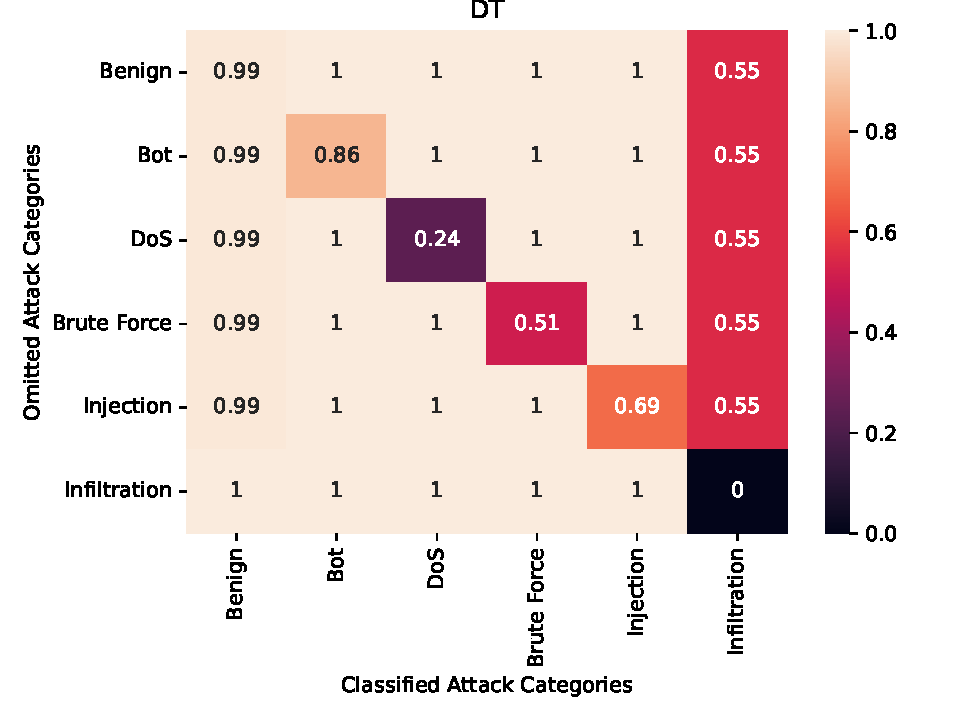
\includegraphics[width=\textwidth,keepaspectratio]{dt_exc_category}
    \end{minipage}\hfill
    \begin{minipage}[h]{0.5\textwidth}
        \centering
        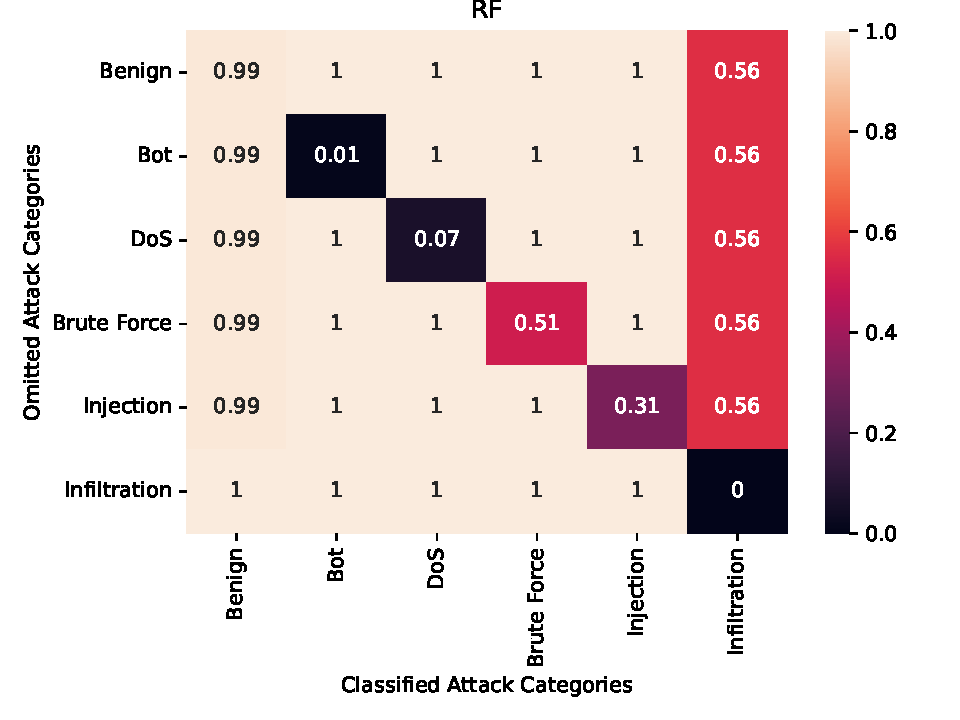
\includegraphics[width=\textwidth,keepaspectratio]{rf_exc_category}
    \end{minipage}
    %
    \begin{minipage}[h]{0.5\textwidth}
        \centering
        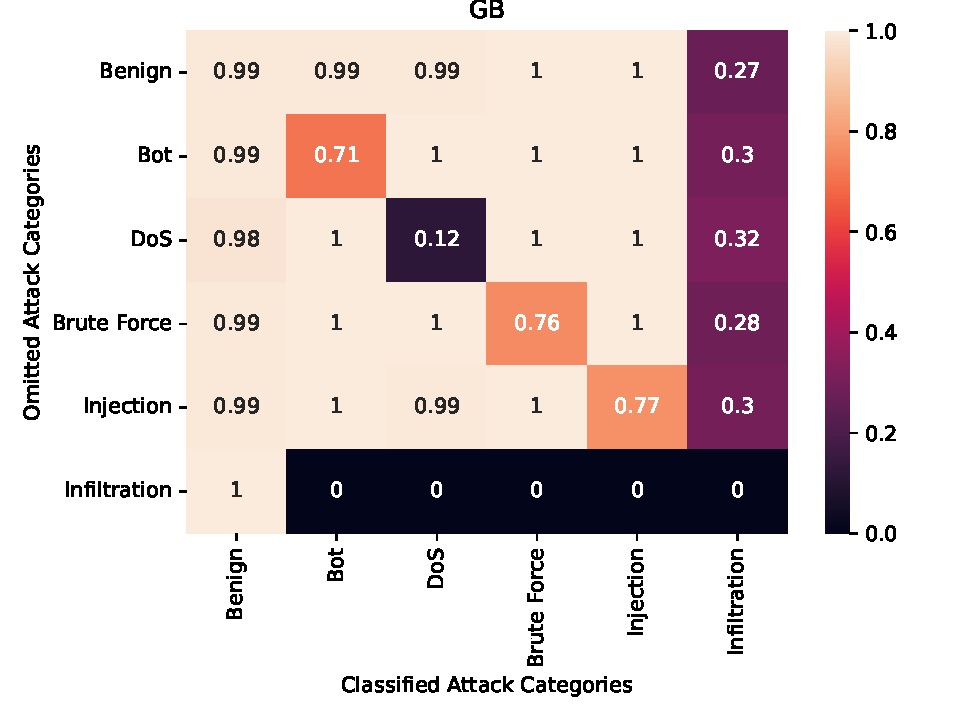
\includegraphics[width=\textwidth,keepaspectratio]{gb_exc_category}
    \end{minipage}\hfill
    \begin{minipage}[h]{0.5\textwidth}
        \centering
        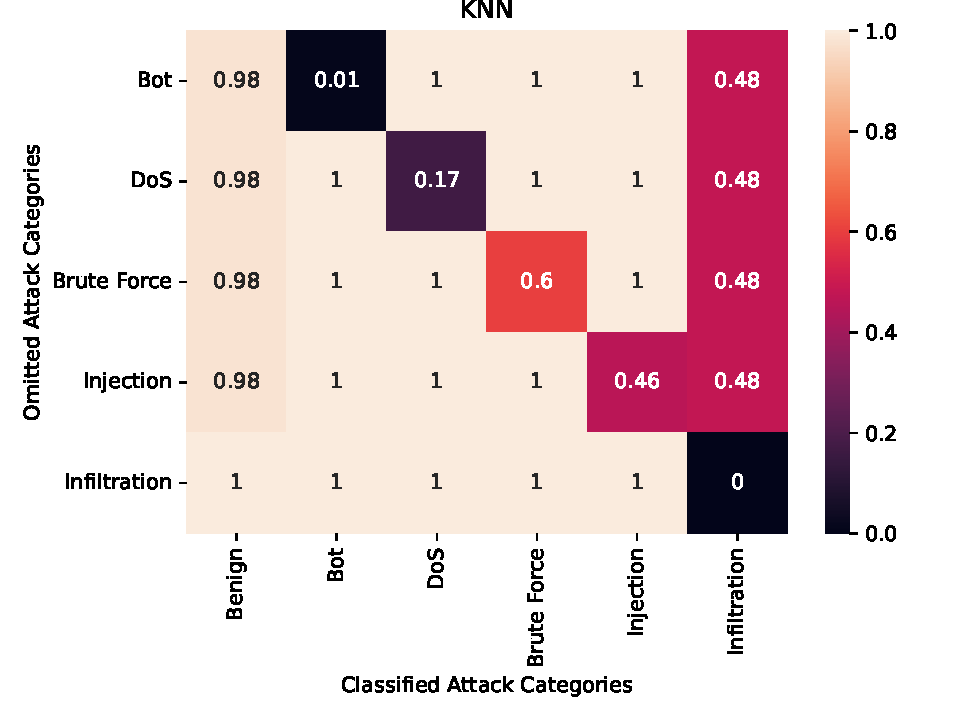
\includegraphics[width=\textwidth,keepaspectratio]{knn_exc_category}
    \end{minipage}
    \begin{minipage}[h]{0.5\textwidth}
        \centering
        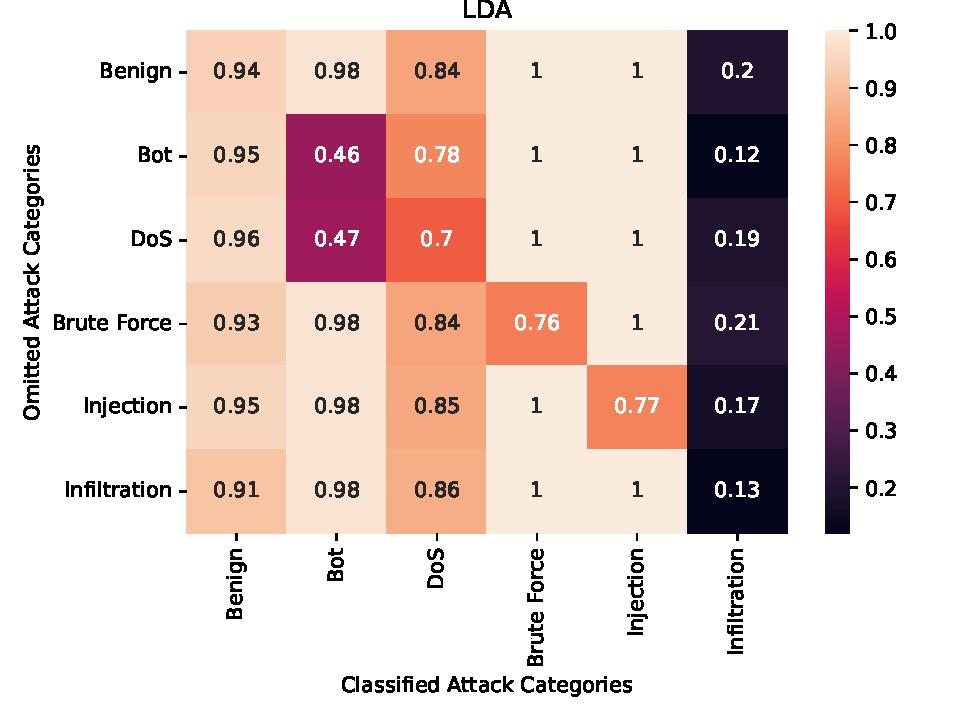
\includegraphics[width=\textwidth,keepaspectratio]{lda_exc_category}
    \end{minipage}
    \caption[Category Omission Results]{Recall values per class when trained on variants omitting a single category.\label{fig:exc_cat}}
\end{figure}
% 
Figure~\ref{fig:exc_cat} shows the heatmaps of recall values of the supervised
models generated from the variants omitting categories. Each row represents the
per category recall values generated from one variant. The label of the row is
the category that was omitted.

The results in these heatmaps further confirm the observations made earlier on
the high efficacy of supervised models on known attacks and reduced efficacy on
unknown attacks, indicated by the lower diagonal values. The \gls{dt}, \gls{rf}
and \gls{knn} models seem to behave similarly, performing excellently on known
attacks but more poorly on unknown attacks, with \gls{dt} demonstrating
slightly higher generalisation ability compared to the other models. The
\gls{lda} model differs slightly, exhibiting higher generalisation ability but
slightly lower values overall and significantly lower values on the
`Infiltration' category specifically. The \gls{gb} model exhibits strange
behaviour as it seems to be dependent on the `Infiltration' category to learn
patterns on the other classes, achieving zero recall values when the category
is excluded. Paradoxically, the model also displays lower recall on the
`Infiltration' category compared to the other models.
%
\begin{figure}[htbp]
    \centering
    \begin{minipage}[h]{0.5\textwidth}
        \centering
        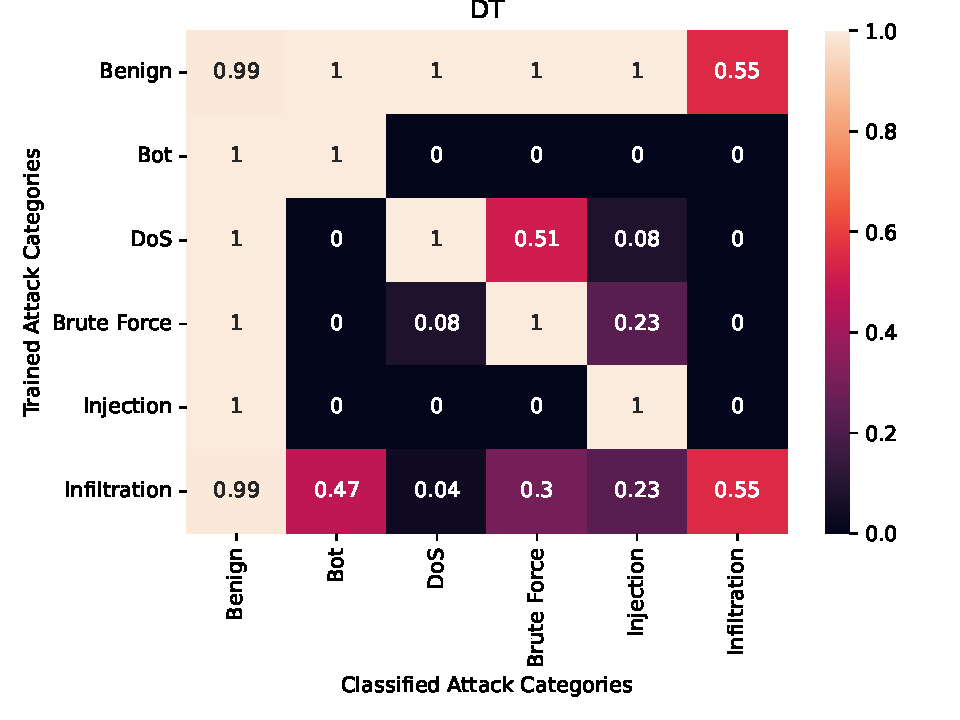
\includegraphics[width=\textwidth,keepaspectratio]{dt_inc_category}
    \end{minipage}\hfill
    \begin{minipage}[h]{0.5\textwidth}
        \centering
        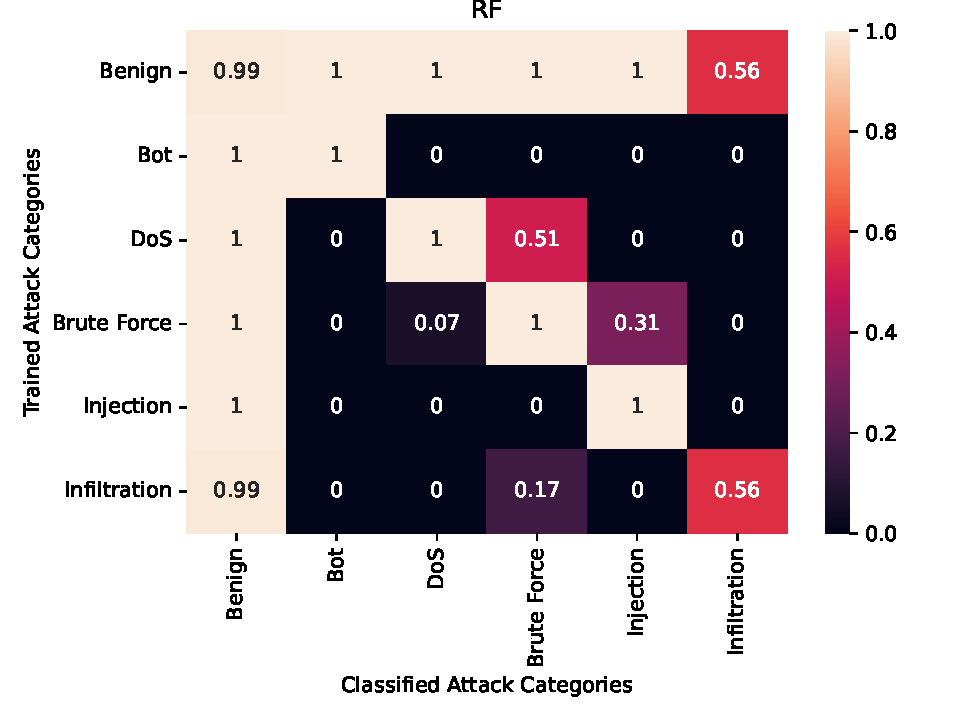
\includegraphics[width=\textwidth,keepaspectratio]{rf_inc_category}
    \end{minipage}
    %
    \begin{minipage}[h]{0.5\textwidth}
        \centering
        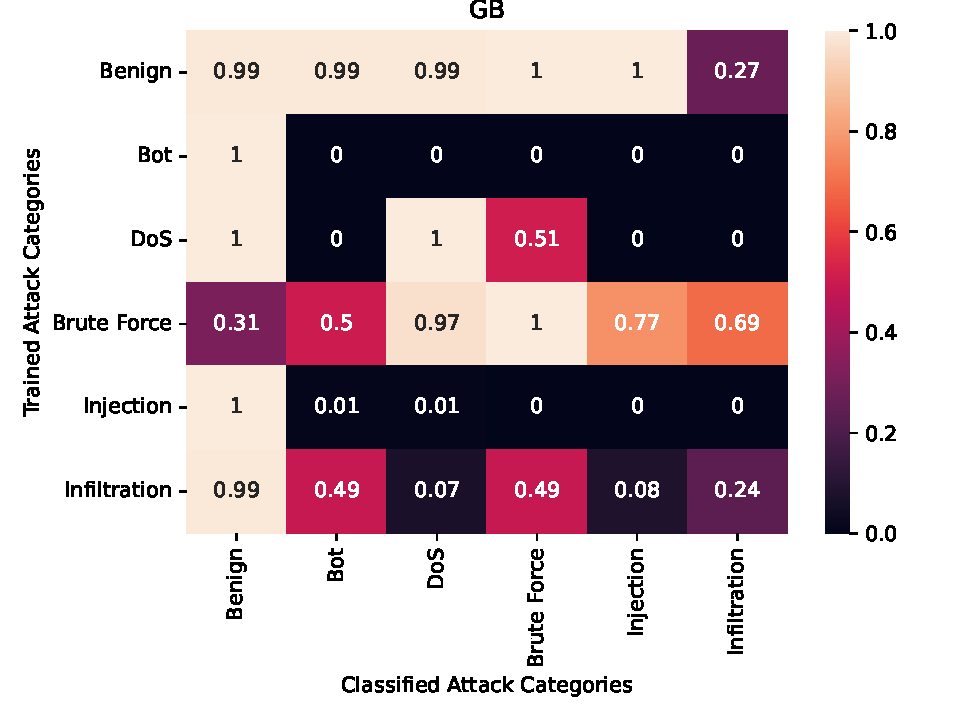
\includegraphics[width=\textwidth,keepaspectratio]{gb_inc_category}
    \end{minipage}\hfill
    \begin{minipage}[h]{0.5\textwidth}
        \centering
        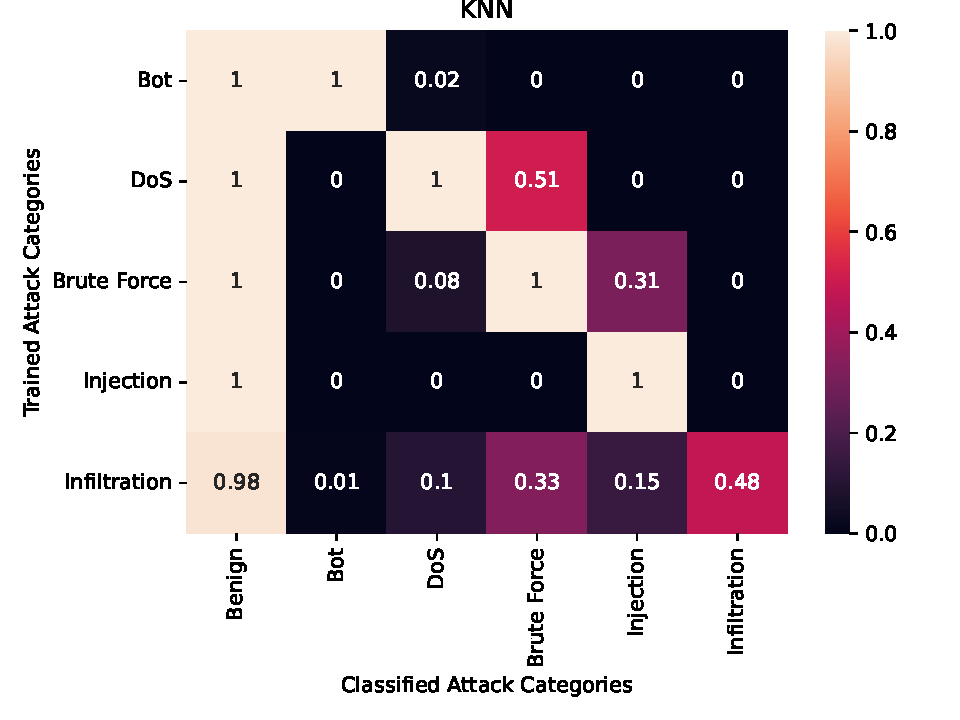
\includegraphics[width=\textwidth,keepaspectratio]{knn_inc_category}
    \end{minipage}
    \begin{minipage}[h]{0.5\textwidth}
        \centering
        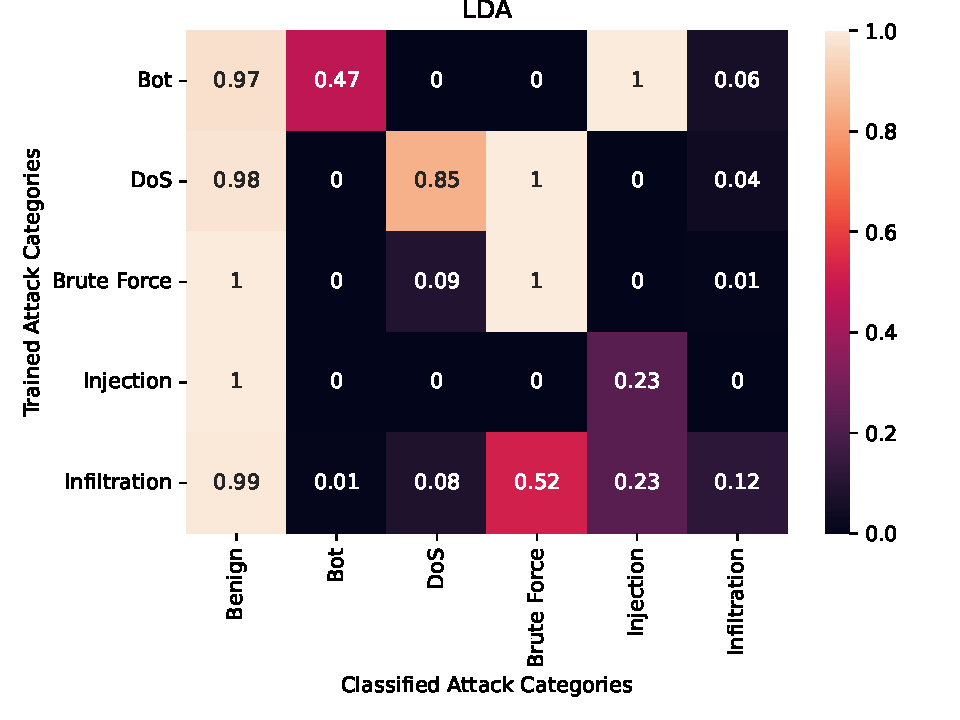
\includegraphics[width=\textwidth,keepaspectratio]{lda_inc_category}
    \end{minipage}
    \caption[Single Category Results]{Recall values per class when trained on a single category.\label{fig:inc_cat}}
\end{figure}

% TODO: continue new model revision from here
This strange behaviour can be further explored in Figure~\ref{fig:inc_cat},
which shows the heatmaps of recall values generated from the variants including
single categories. Based on the values presented in this heatmap, the \gls{gb}
model seems to be able to learn patterns that allow it to generalise from the
`Brute Force' and `Infiltration' categories, but fails to learn anything from
the `Bot' and `Injection' categories. This is in contrast with the \gls{dt},
\gls{rf} and \gls{knn} models, which are able to learn from all categories,
indicated by the high recall values in the diagonal, however are not able to
generalise when trained on `Brute Force' attacks. The \gls{lda} model displays
lower values in the diagonal and generalises similarly to the other models
excluding the \gls{gb} model. This indicates lower performance overall when
trained on single attacks.

All classifiers except for the \gls{rf} classifier seem to be able to
generalise from the `Infiltration' class. This behaviour, in conjunction with
the previous observations on the low accuracy on this class supports the idea
that the `Infiltration' category may be too broad and contain more than one
sort of attack. This would explain why it is difficult to classify, yet offers
information about a wide variety of attacks.

Despite these limited instances of generalisation, the overall generalisation
ability of the five models is low. Most instances of generalisation on this set
of heatmaps yield low recall values, with the diagonal containing significantly
higher values indicating a limited ability to generalise across categories
overall.

\section{Per Variant Results Omitting Specific Attacks}%
\label{sec:res_var_att}

%
\begin{figure}[htbp]
    \centering
    \begin{minipage}[h]{0.5\textwidth}
        \centering
        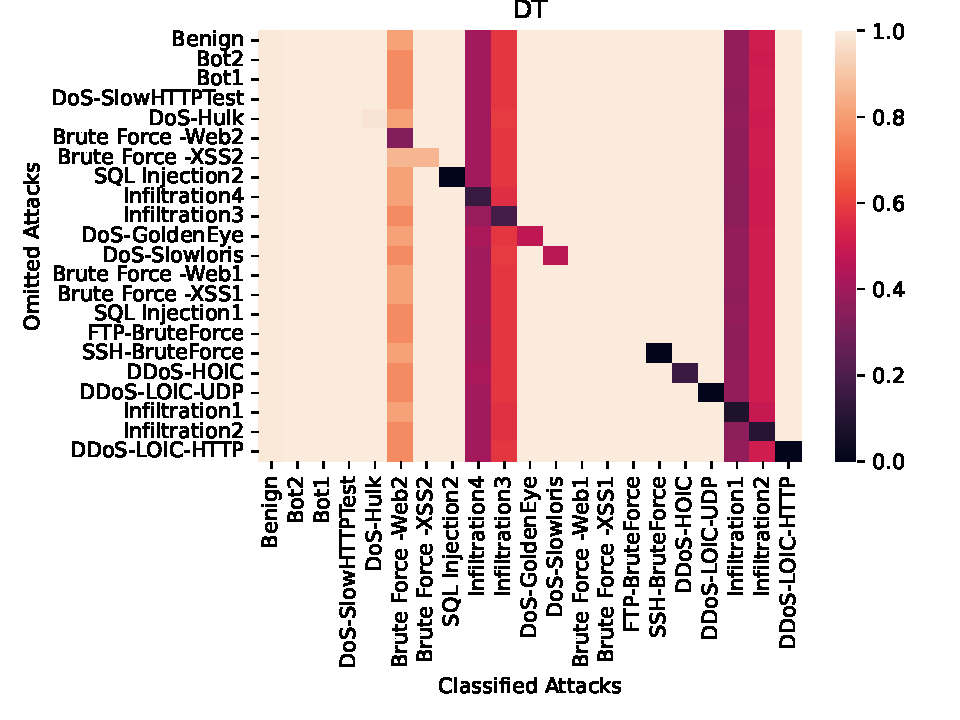
\includegraphics[width=\textwidth,keepaspectratio]{dt_exc_attack}
    \end{minipage}\hfill
    \begin{minipage}[h]{0.5\textwidth}
        \centering
        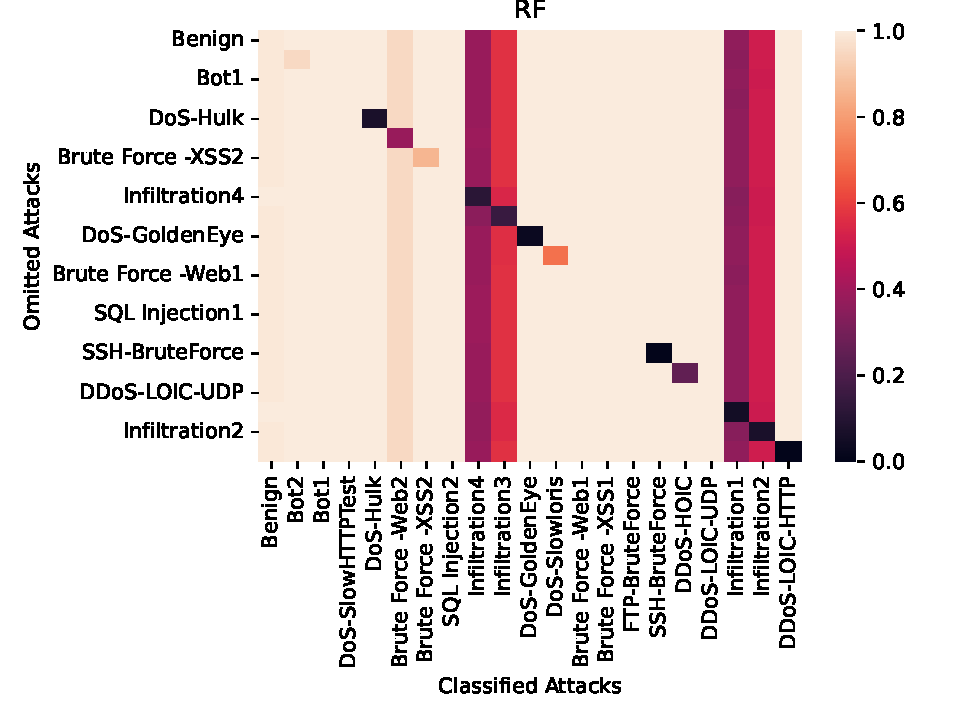
\includegraphics[width=\textwidth,keepaspectratio]{rf_exc_attack}
    \end{minipage}
    %
    \begin{minipage}[h]{0.5\textwidth}
        \centering
        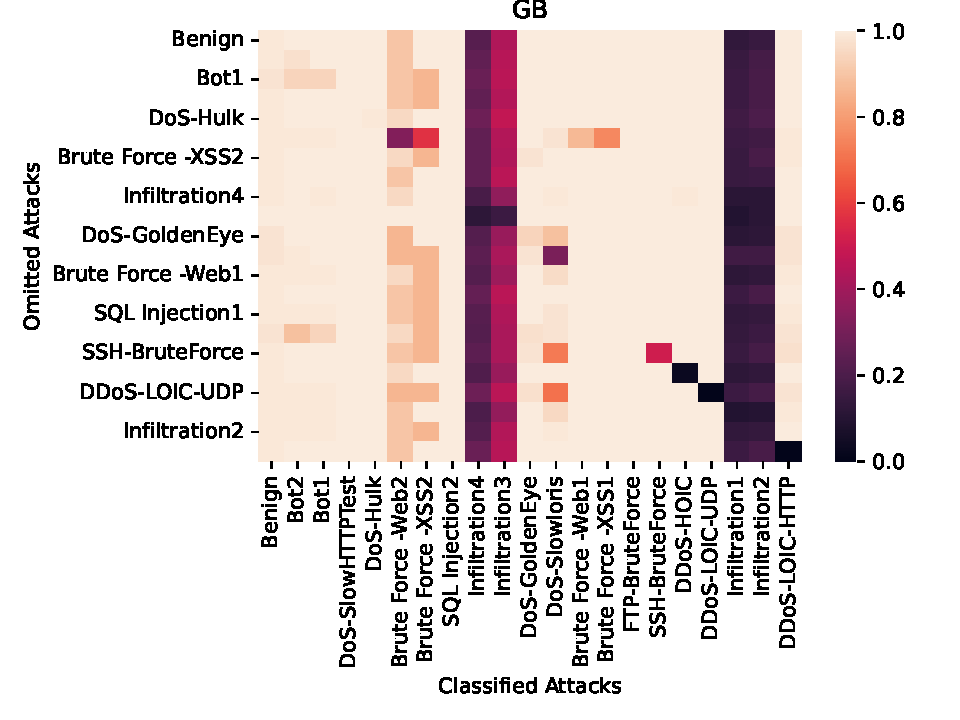
\includegraphics[width=\textwidth,keepaspectratio]{gb_exc_attack}
    \end{minipage}\hfill
    \begin{minipage}[h]{0.5\textwidth}
        \centering
        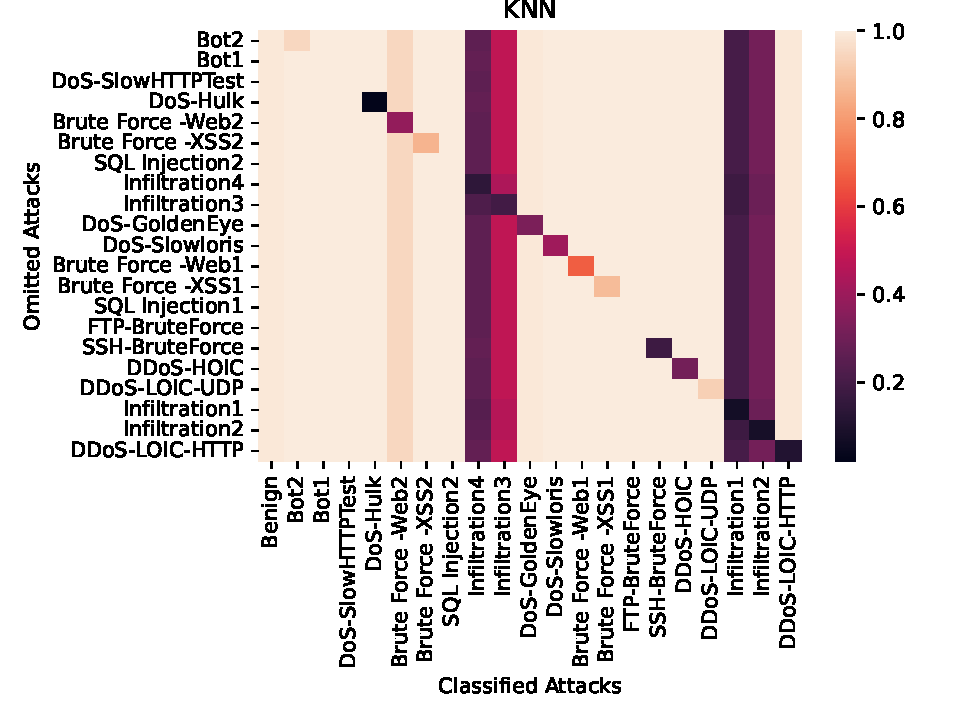
\includegraphics[width=\textwidth,keepaspectratio]{knn_exc_attack}
    \end{minipage}
    \begin{minipage}[h]{0.5\textwidth}
        \centering
        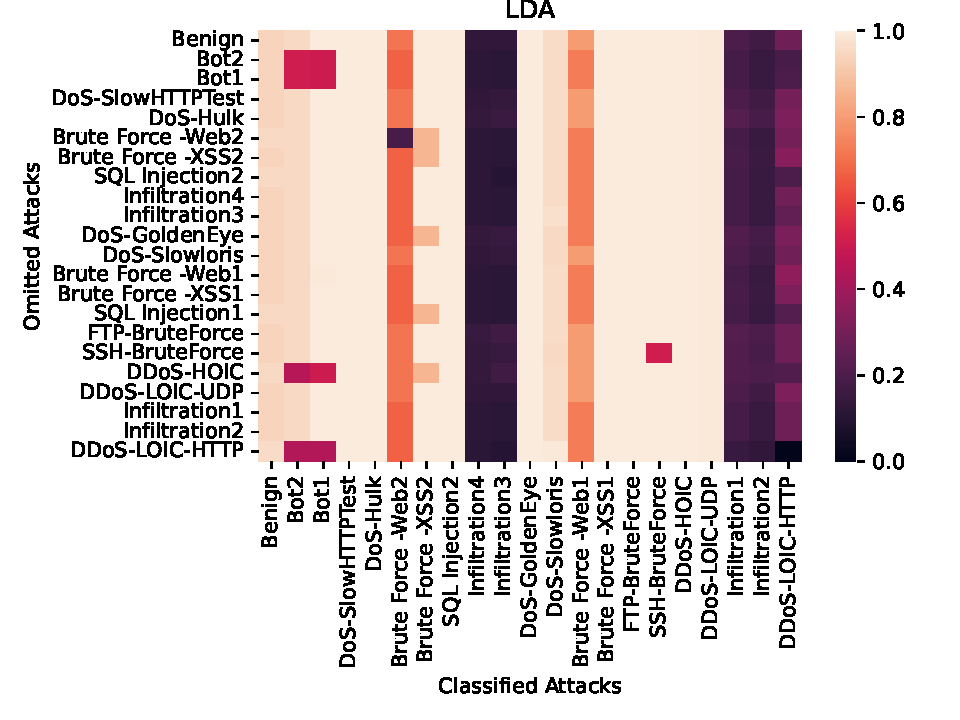
\includegraphics[width=\textwidth,keepaspectratio]{lda_exc_attack}
    \end{minipage}
    \caption[Individual Attack Omission Results.]{Recall values per class when trained on variants omitting a single attack.\label{fig:exc_att}}
\end{figure}
%
Figure~\ref{fig:exc_att} shows the heatmaps of recall values of the supervised
models generated from the variants omitting individual attacks. Each row
represents the per attack recall values generated from one variant. The label
of the row is the attack that was omitted.

The primary patterns to observe are the vertical stripes wherever
`Infiltration' attacks are present and the diagonal, representing the
difficulty of classifying `Infiltration' attacks and generalising to unknown
attacks. It is interesting to note, the diagonals have gaps, unlike in the
category heatmaps. This indicates intra-category generalisation occurs during
training, creating these gaps that are not visible in the category heatmaps.
The slightly more noisy heatmaps resulting from the \gls{gb} model is further
evidence this model is more dependent on generalised patterns compared to the
other models. The \gls{lda} model also exhibits a slightly noisier heatmap
however to a much lower degree than the \gls{gb} model.

\begin{figure}[htbp]
    \centering
    \begin{minipage}[h]{0.5\textwidth}
        \centering
        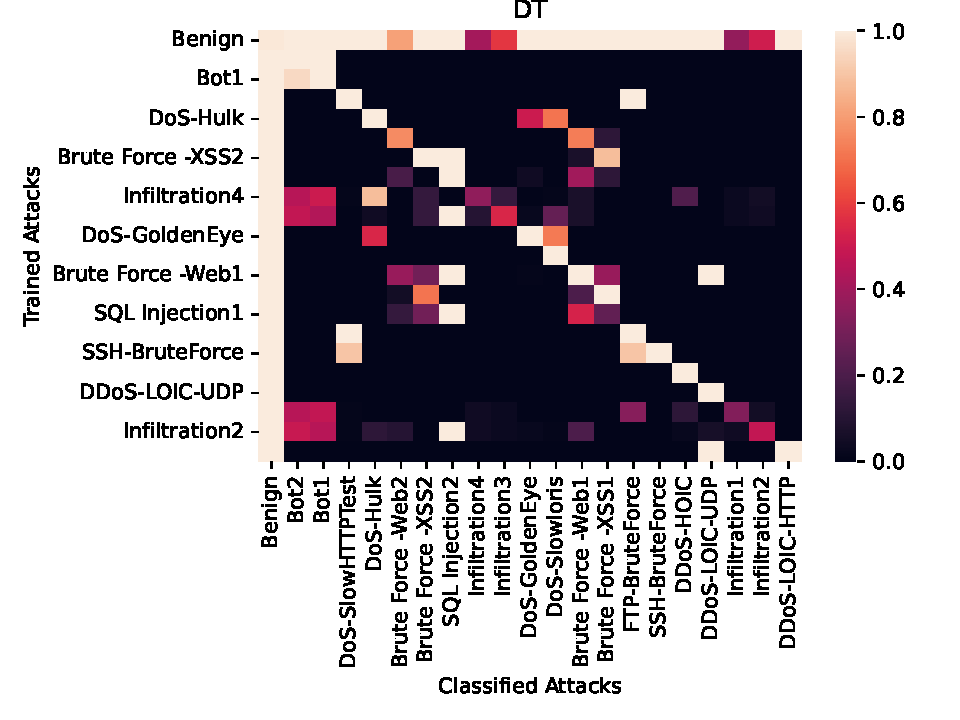
\includegraphics[width=\textwidth,keepaspectratio]{dt_inc_attack}
    \end{minipage}\hfill
    \begin{minipage}[h]{0.5\textwidth}
        \centering
        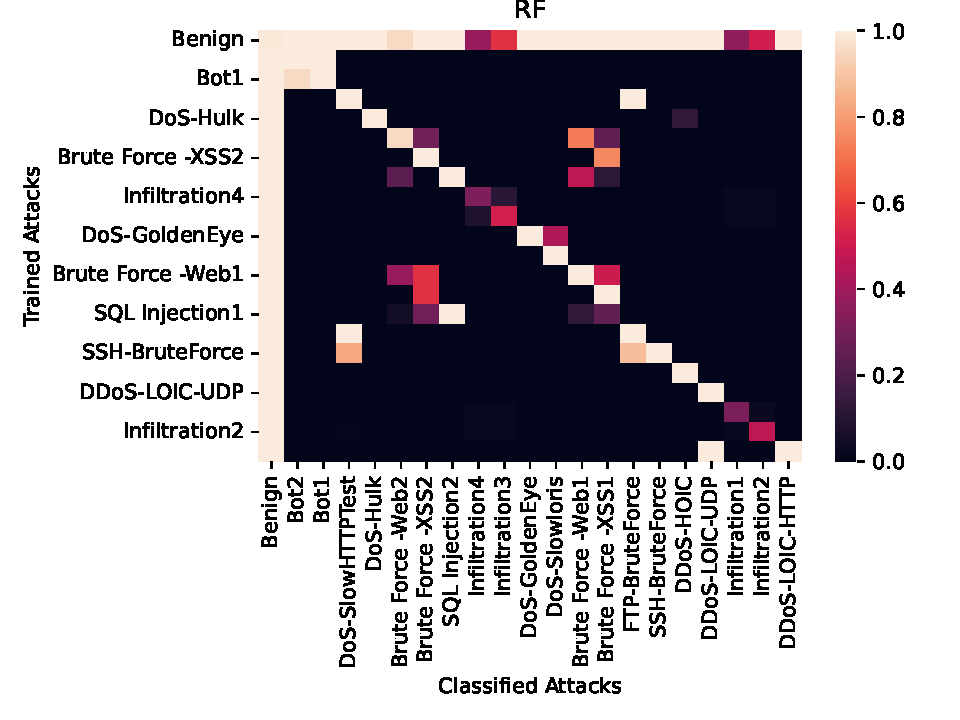
\includegraphics[width=\textwidth,keepaspectratio]{rf_inc_attack}
    \end{minipage}
    %
    \begin{minipage}[h]{0.5\textwidth}
        \centering
        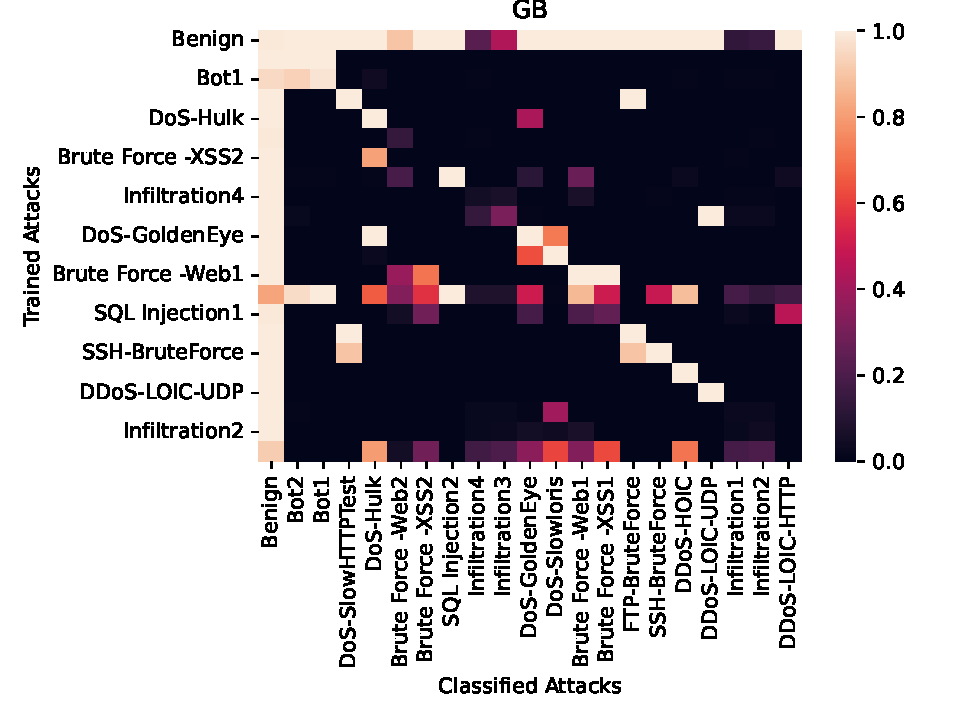
\includegraphics[width=\textwidth,keepaspectratio]{gb_inc_attack}
    \end{minipage}\hfill
    \begin{minipage}[h]{0.5\textwidth}
        \centering
        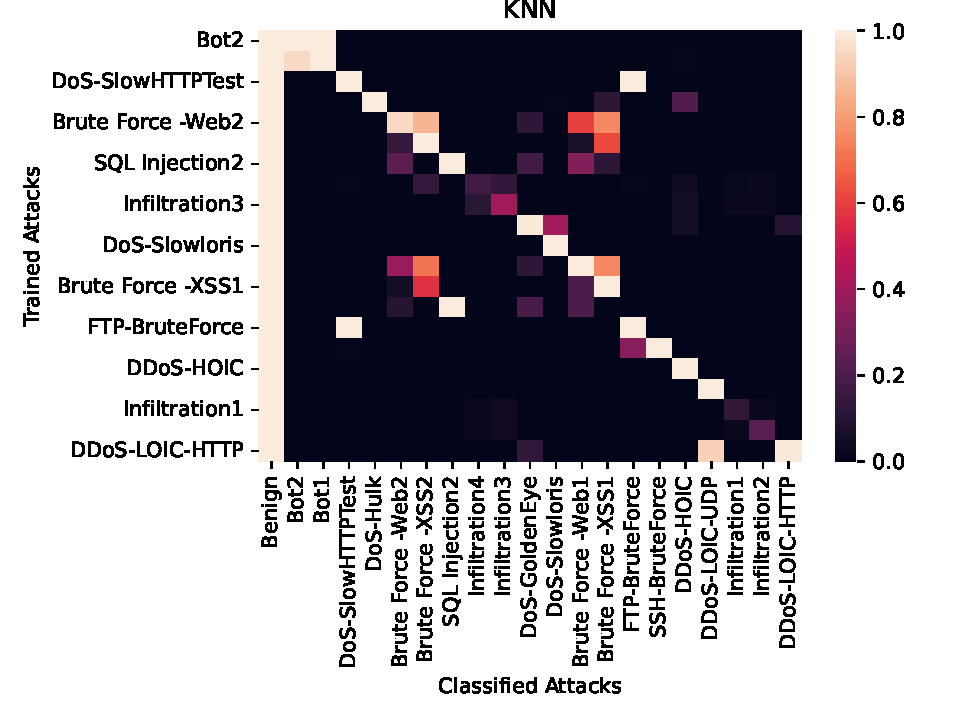
\includegraphics[width=\textwidth,keepaspectratio]{knn_inc_attack}
    \end{minipage}
    \begin{minipage}[h]{0.5\textwidth}
        \centering
        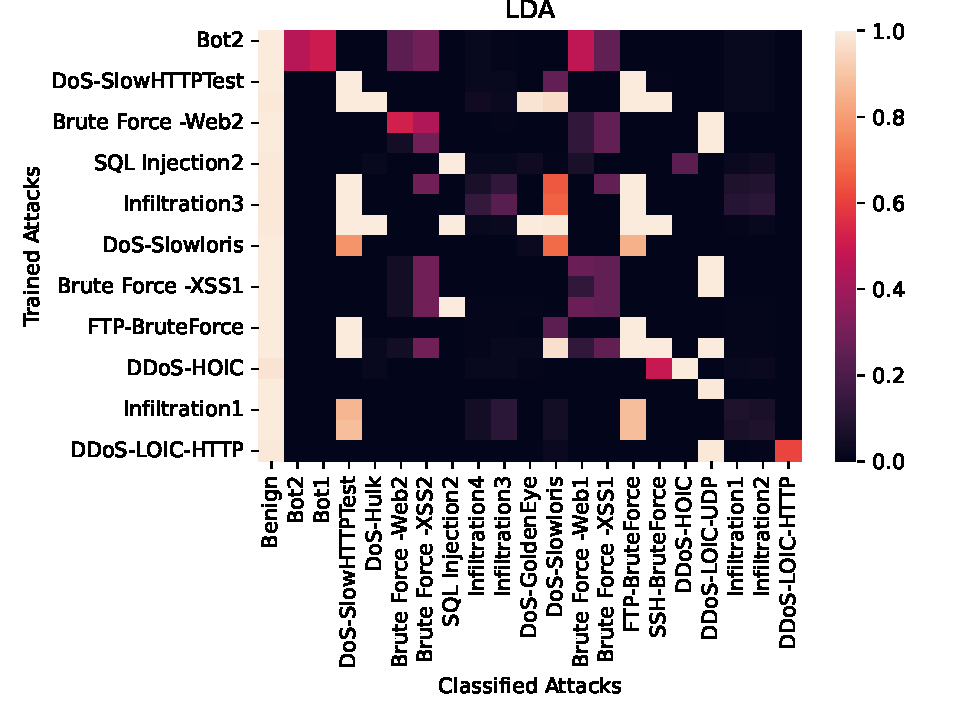
\includegraphics[width=\textwidth,keepaspectratio]{lda_inc_attack}
    \end{minipage}
    \caption[Single Individual Attack Results]{Recall values per class when trained on a single attack.\label{fig:inc_att}}
\end{figure}
%

Figure~\ref{fig:inc_att} shows the heatmaps of recall values generated from the
variants including single attacks. These results indicate that while
generalisation is somewhat scarce, there are numerous attacks in the dataset
that influence the model's performance on other attacks. The relationships
between each pair of attacks are indicated in the heatmaps. It should be noted
that the algorithm employed seems to have a significant effect on the level of
generalisation achieved, with \gls{gb}, \gls{dt} and \gls{lda} demonstrating
the higher generalisation ability than \gls{rf} and \gls{knn}.

\section{Addressing Objectives}%
\label{sec:add_obj}

Sections~\ref{sec:agg_res_cat} and~\ref{sec:agg_res_att} contain all the
information required to address \hyperlink{obj}{Objective 1}. The
state-of-the-art supervised models considered demonstrate impressive efficacy
in detecting known network intrusions, however, their efficacy diminishes to an
alarming degree when faced with unknown attacks. Hence, their overall efficacy
will depend on the types of attacks the system is expected to face, and the
dataset available for training. The state-of-the-art unsupervised models
considered exhibit far lower efficacy, however, experience negligible decline
against unknown attacks. This may offer an invaluable tool in flagging
potentially malicious behaviour, however, may not be suitable if a high degree
of confidence in predictions is required.

The same sections also detail enough information to address
\hyperlink{obj}{Objective 2}, it is clear to see that the supervised models
considered are more effective overall, performing better in all metrics except
for Recall-Unk. However, unsupervised models are significantly more effective
in detecting unknown attacks.

The heatmaps presented in Figures~\ref{fig:inc_cat} and~\ref{fig:inc_att}
address \hyperlink{obj}{Objective 3}, clearly illustrating the relationships
between attack categories and individual attacks that allow the different
\gls{ml} models to generalise across classes.

\section{Threats to Validity}%
\label{sec:threats}
It should be noted from the results, that the unsupervised models perform much
better on the NSL-KDD dataset than the CSE-CIC-IDS2018 dataset. This highlights
the issue of generalisation across datasets. The unsupervised models considered
were selected as they were the most highly cited and best performing models
within the domain that provide a clear methodology from the models found during
the literature review. This implicitly assumes that the high efficacy
demonstrated on the NSL-KDD dataset and the other datasets they were evaluated
on, generalises well to the CSE-CIC-IDS2018 dataset, which may not always be
the case. Hence, it is possible these models are not the best performing models
on the dataset considered for this study, resulting in an unfair comparison
with the supervised models.

Furthermore, the issue of cross-dataset generalisation also brings into
question how well these results will truly generalise outside the lab
environment. Whilst, to the best of our knowledge, the CSE-CIC-IDS2018 dataset
is the most up-to-date and realistic dataset currently available, it may still
not generalise well to other datasets and practical environments.

As mentioned in Section~\ref{sec:preprocessing} the individual attack labels
were generated based on the timestamp and label information in Table 2 of the
CSE-CIC-IDS2018 website~\cite{cic2018}. It was also mentioned that some attack
instances are dated outside the range of any attack listed on the table, and it
has therefore been assumed that instances occurring on a date with only one
attack of that label, belong to that attack. This assumption, whilst likely the
most logical approach, may lead to the mislabelling of certain samples.
Measuring the likelihood of this or mitigating the issues is difficult without
more information on the source of the ambiguous samples, which does not appear
to be available in the resources documenting the dataset.

Finally, all pragmatic cyberthreat defence systems present vulnerabilities of
their own which should be kept in mind when considering results. The
CSE-CIC-IDS2018 dataset was not designed with the \gls{nids} components
employed by this study in mind. Hence, the attacks it contains were performed
without any knowledge of the defence system we have employed. In practice,
attackers could learn implementation details of any defence system and
orchestrate targeted attacks intended to circumvent that specific defence
system. A prime example of such an attack targeted at \gls{ml}-based \gls{nids}
are adversarial attacks, which are attacks intentionally designed to evade
\gls{ml}-based classifiers.~\cite{adversarial1} and~\cite{adversarial2} propose
examples of such attack tools.

\section{Conclusion}%
\label{sec:conclusion4}

In this chapter, we have presented the results of our replicated models both on
datasets used by the original authors and on the variants of the
CSE-CIC-IDS2018 dataset generated from the methodology discussed in the
previous chapter. These results address all three objectives originally defined
in Chapter~\ref{chp:introduction} and provide valuable insights into the
strengths and weaknesses of different machine learning techniques in the face
of both known and unknown attacks. In the next chapter, we conclude the
document, summarising are key points and proposing future research directions.